\documentclass[aspectratio=169]{beamer}

% Tema portable: solo paquetes de una instalacion LaTeX estandar (sin fuentes
% externas), para compilar con tectonic / texlive / pdflatex sin extras.
\usetheme{Madrid}
\usecolortheme{whale}
\useinnertheme{circles}
\beamertemplatenavigationsymbolsempty

\usepackage[utf8]{inputenc}
\usepackage[T1]{fontenc}
\usepackage[spanish]{babel}
\usepackage{graphicx}
\usepackage{booktabs}
\usepackage{xcolor}

\graphicspath{{figs/}}

\title[vectorjobs]{vectorjobs --- Estado actual}
\subtitle{Centroides, valor de mercado y costos de cómputo}
\author{Equipo vectorjobs}
\institute{Pipeline de recomendación job\,$\leftrightarrow$\,skill}
\date{18 de junio de 2026}

\begin{document}

\begin{frame}
  \titlepage
\end{frame}

\begin{frame}{Agenda}
  \tableofcontents
\end{frame}

% ------------------------------------------------------------------ %
\section{Contexto y estado actual}

\begin{frame}{¿Qué es vectorjobs?}
  \begin{itemize}
    \item Pipeline que convierte postings de LinkedIn (\textbf{123.849 jobs},
          abril 2024) en un dataset \emph{silver} reproducible.
    \item Recomendación job\,$\leftrightarrow$\,skill con varios backends:
      \begin{itemize}
        \item \textbf{TF-IDF / SVD} --- baseline disperso, CPU.
        \item \textbf{Qwen3-Embedding-0.6B} --- denso, GPU opcional.
        \item \textbf{Mock} --- backend determinista para tests.
      \end{itemize}
    \item Analítica temporal: deriva de centroides, evolución de skills,
          clustering interpretable y curvas de supervivencia.
  \end{itemize}
  \vfill
  \footnotesize Fuente de datos: Kaggle \texttt{arshkon/linkedin-job-postings}.
\end{frame}

\begin{frame}{Estado actual --- madurez M2.3}
  \begin{columns}[T]
    \begin{column}{0.5\textwidth}
      \textbf{Arquitectura de datos}
      \begin{itemize}
        \item \texttt{raw} (CSV Kaggle) $\rightarrow$
        \item \texttt{silver} (Parquet, \texttt{job\_card\_text}) $\rightarrow$
        \item \texttt{gold} (embeddings + índices)
      \end{itemize}
    \end{column}
    \begin{column}{0.5\textwidth}
      \textbf{Hecho}
      \begin{itemize}
        \item Clusters fijos (k=12) con centroides diarios para el MVP.
        \item Reportes temporales (47 figuras).
        \item Smoke tests semánticos.
      \end{itemize}
      \textbf{Roadmap}
      \begin{itemize}
        \item M3: extracción de skills (Qwen3-8B / vLLM).
        \item M4: métricas de evaluación.
      \end{itemize}
    \end{column}
  \end{columns}
\end{frame}

% ------------------------------------------------------------------ %
\section{La idea de los centroides}

\begin{frame}{Centroides: qué son y por qué importan}
  \begin{columns}[T]
    \begin{column}{0.55\textwidth}
      \begin{itemize}
        \item Cada job es un vector (TF-IDF/SVD o denso).
        \item Un \textbf{centroide} es el vector promedio de un cluster (un
              "sector" del mercado laboral).
        \item Calculamos centroides \textbf{por día} para el MVP y medimos la
              \textbf{deriva} (distancia coseno entre periodos consecutivos).
        \item La deriva $=$ cuánto se mueve el lenguaje/contenido de un sector
              en el tiempo.
      \end{itemize}
    \end{column}
    \begin{column}{0.45\textwidth}
      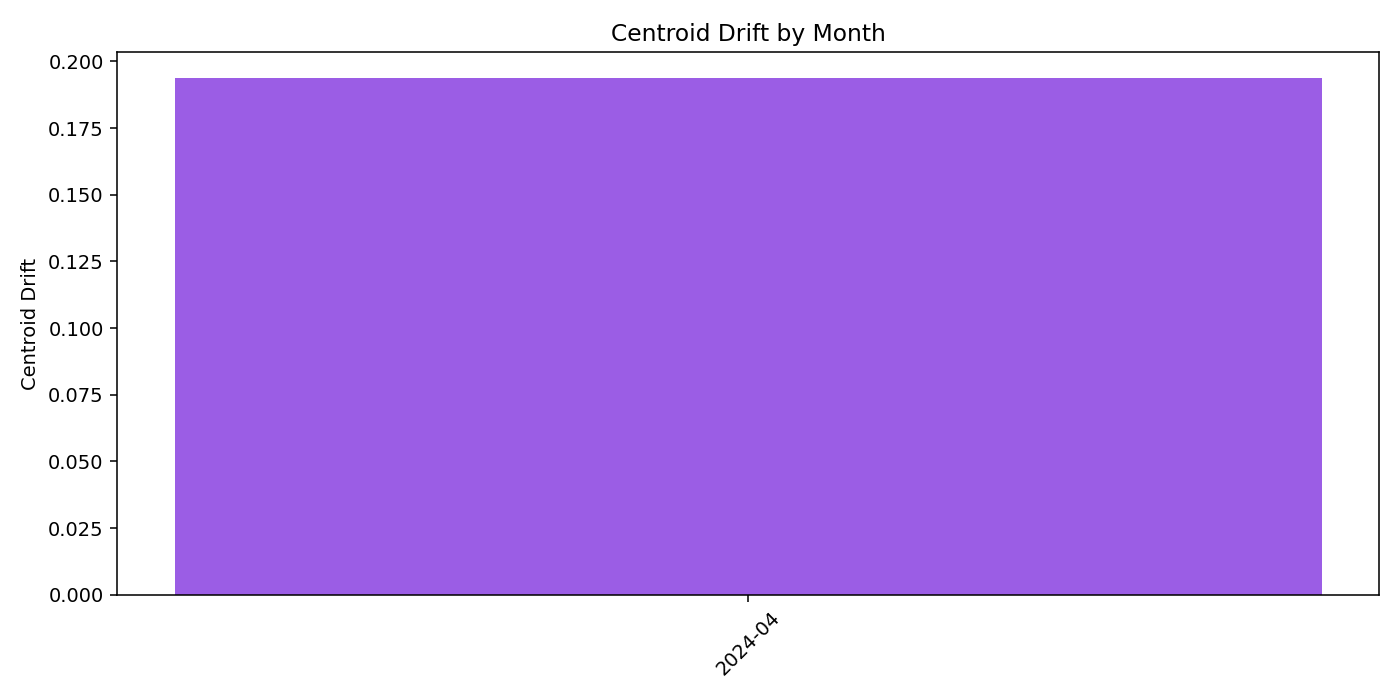
\includegraphics[width=\linewidth]{centroid_drift_by_month.png}
    \end{column}
  \end{columns}
\end{frame}

\begin{frame}{Centroides en el espacio semántico}
  \begin{columns}[T]
    \begin{column}{0.5\textwidth}
      \centering
      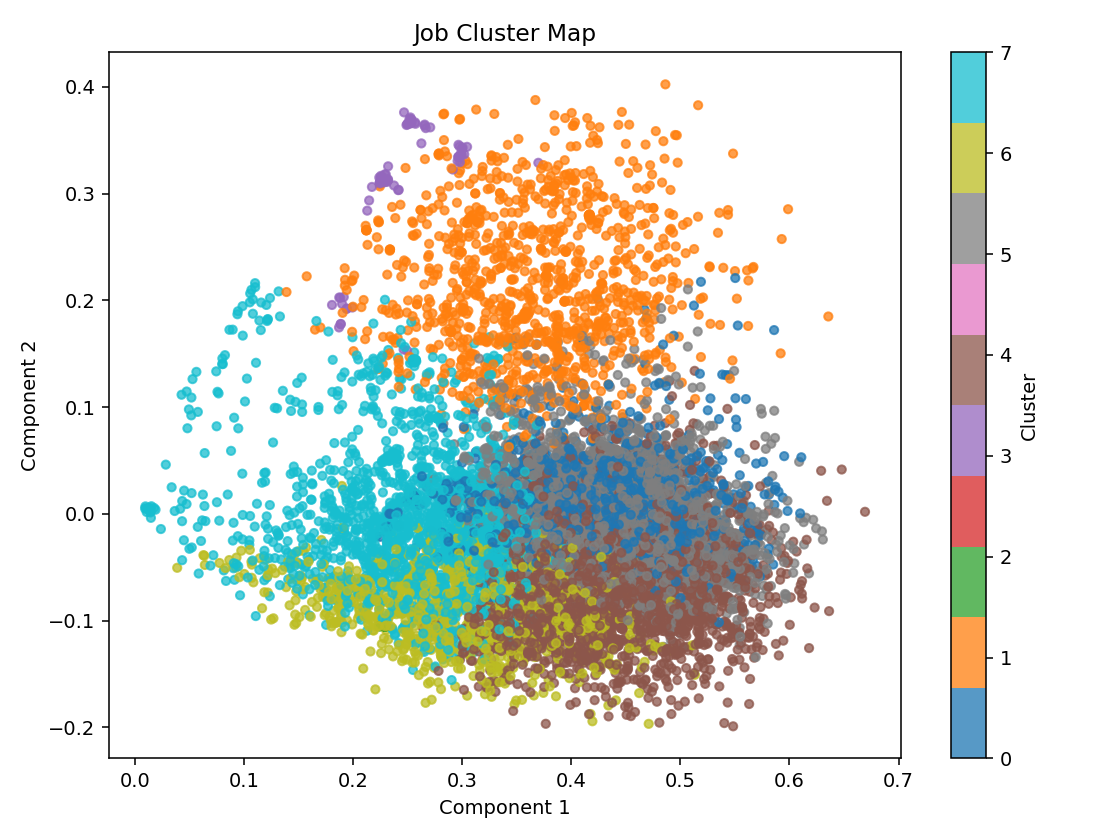
\includegraphics[width=\linewidth]{job_cluster_map_svd.png}\\
      \footnotesize Proyección SVD 2D de los jobs, coloreada por cluster.
    \end{column}
    \begin{column}{0.5\textwidth}
      \centering
      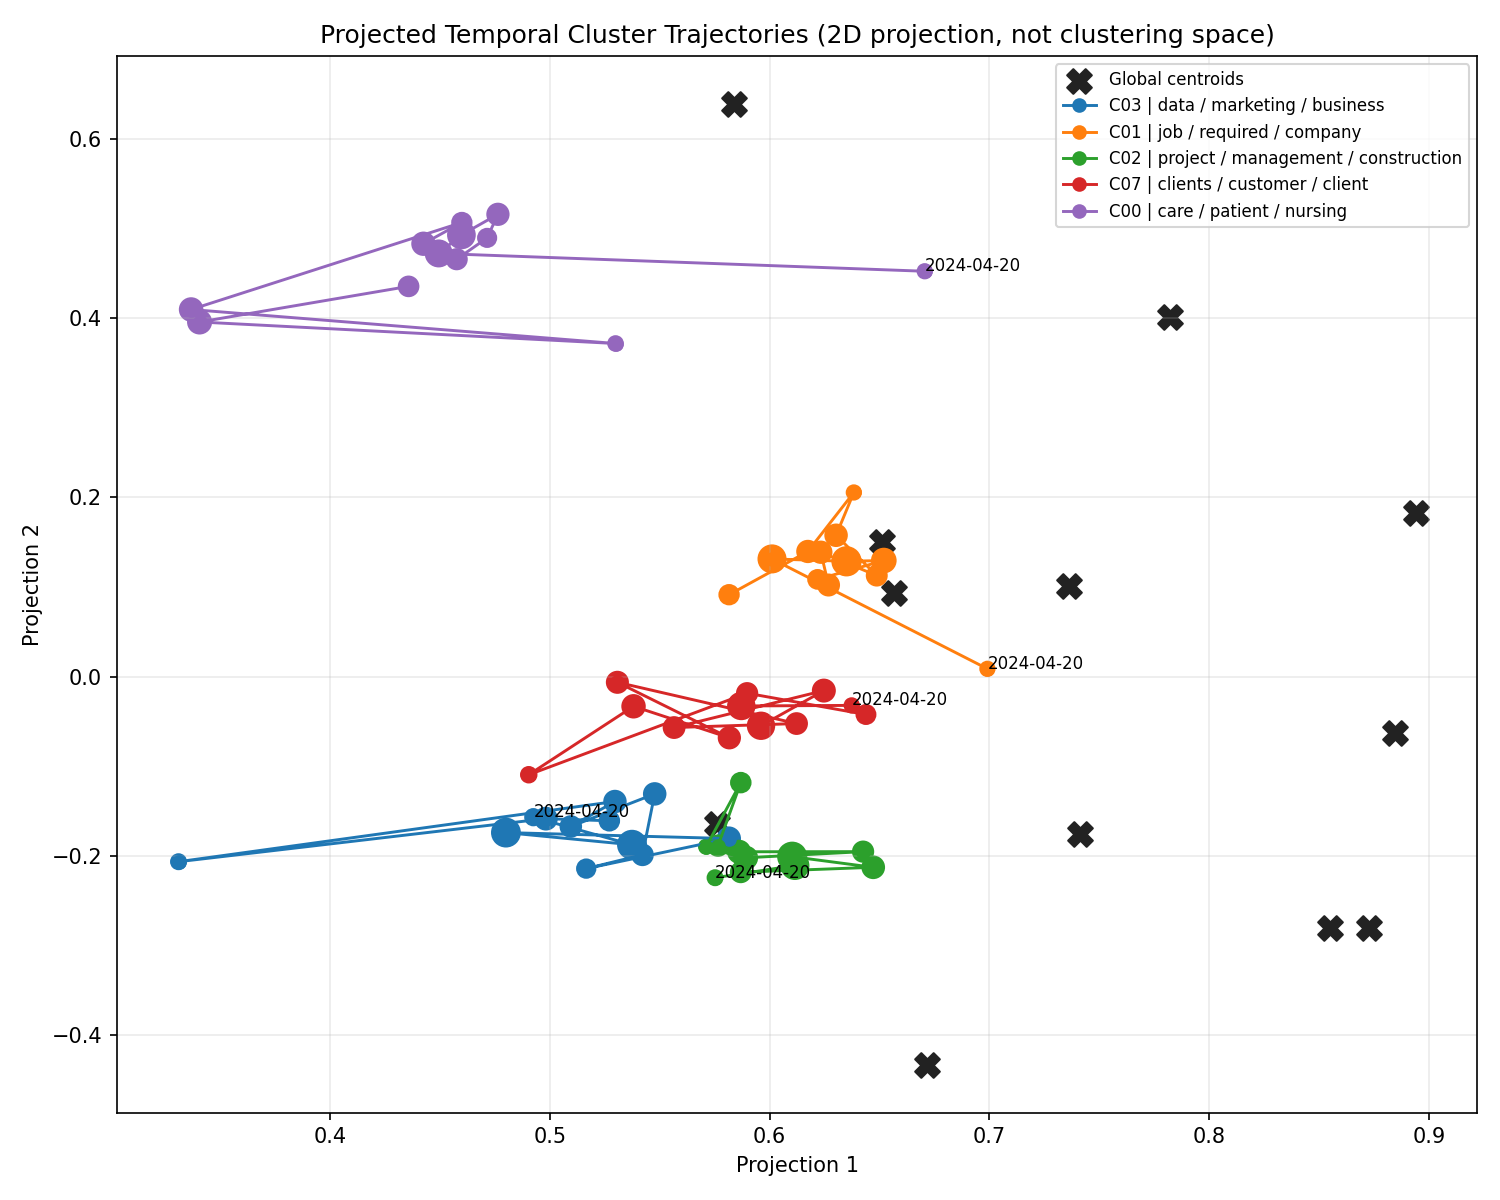
\includegraphics[width=\linewidth]{cluster_semantic_trajectory.png}\\
      \footnotesize Trayectoria semántica de los centroides en el tiempo.
    \end{column}
  \end{columns}
\end{frame}

\begin{frame}{Clusters interpretables (k=12)}
  \begin{columns}[T]
    \begin{column}{0.46\textwidth}
      \scriptsize
      \begin{tabular}{lr}
        \toprule
        Cluster & \#jobs \\
        \midrule
        C03 data / marketing / negocio & 1179 \\
        C01 job / required / company & 1170 \\
        C02 proyecto / gestión / constr. & 1157 \\
        C07 clientes / customer & 1038 \\
        C00 care / patient / nursing & 1036 \\
        C08 sales / business & 818 \\
        C11 design / software / eng. & 787 \\
        \bottomrule
      \end{tabular}
      \vspace{0.5em}\\
      \footnotesize C03 (data/marketing) \textbf{creció} de 11\% a 37\% del share
      en la ventana observada.
    \end{column}
    \begin{column}{0.54\textwidth}
      \centering
      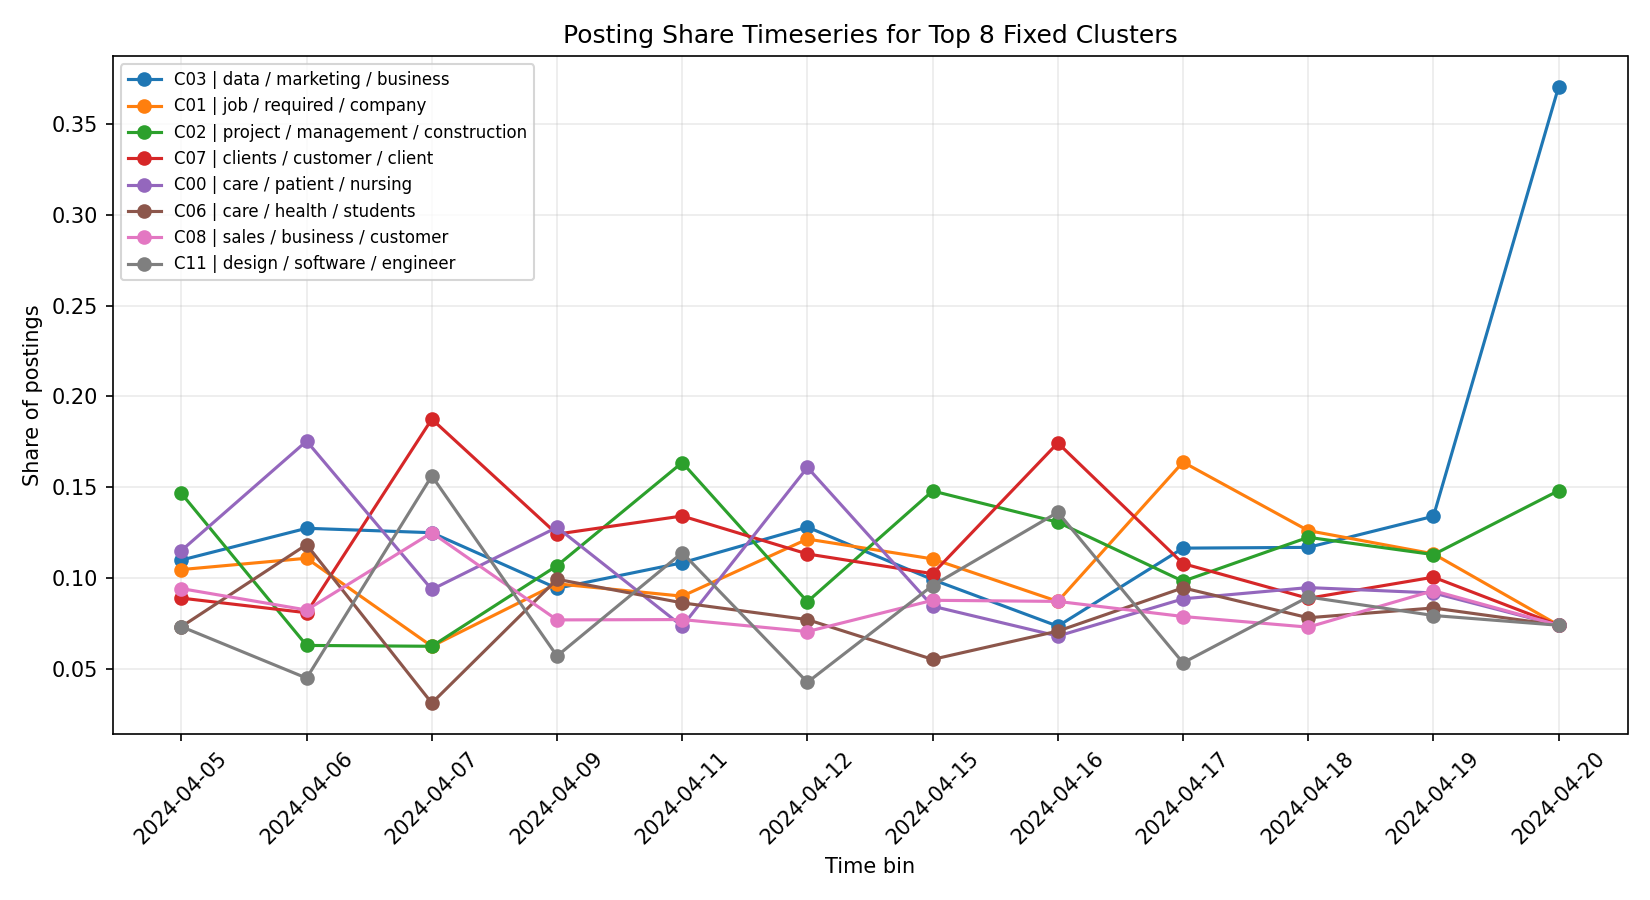
\includegraphics[width=\linewidth]{cluster_share_timeseries.png}\\
      \footnotesize Share de los clusters más grandes a lo largo del tiempo.
    \end{column}
  \end{columns}
\end{frame}

% ------------------------------------------------------------------ %
\section{Valor de mercado en el tiempo}

\begin{frame}{"Market cap" del mercado laboral: volumen $\times$ salario}
  \begin{columns}[T]
    \begin{column}{0.55\textwidth}
      \centering
      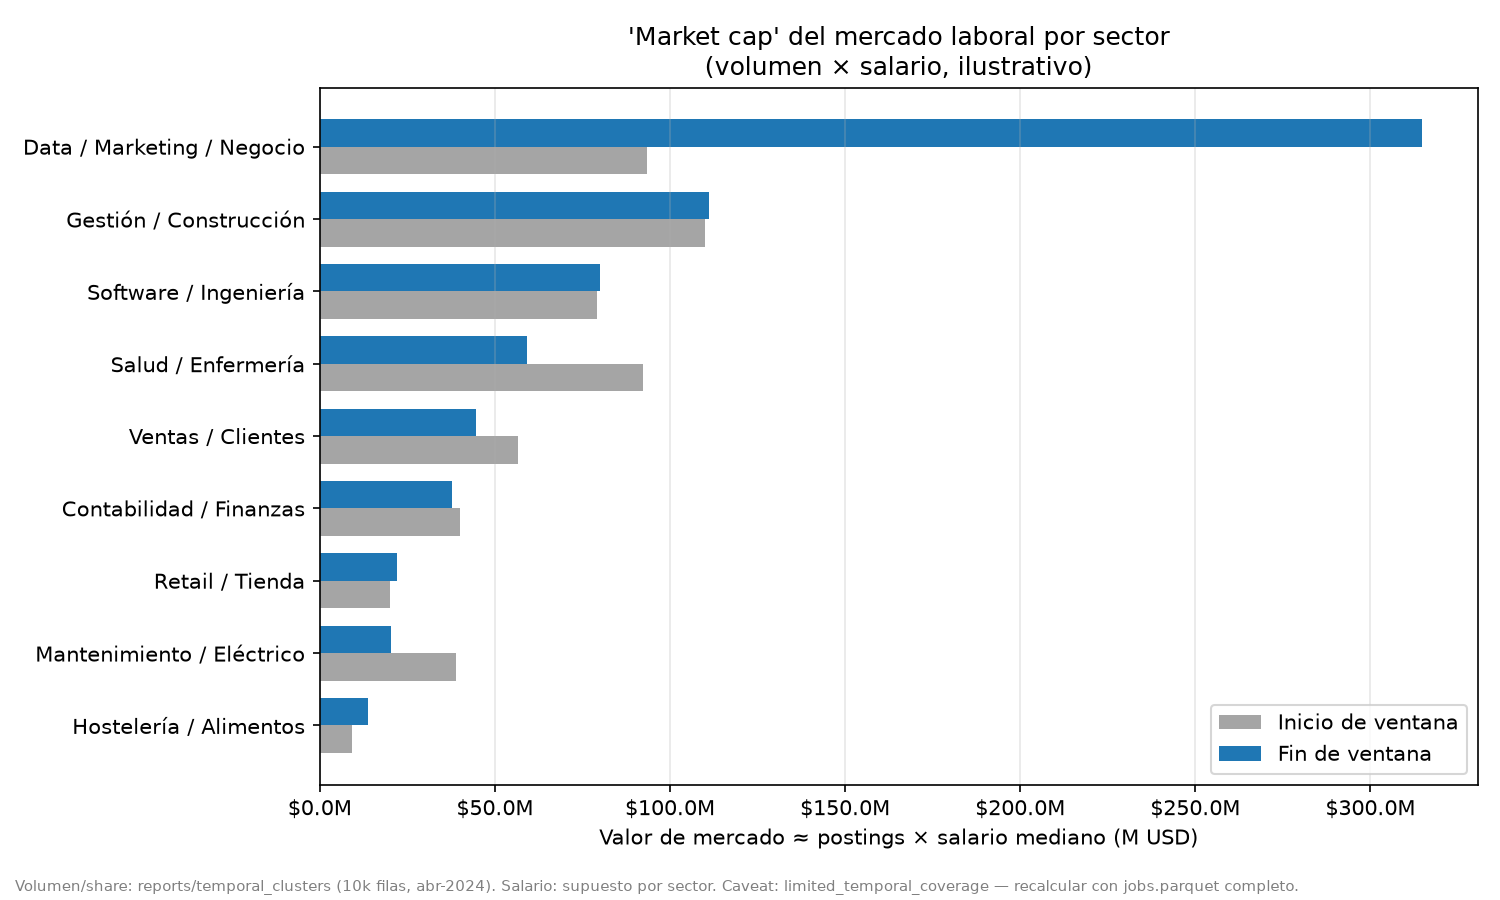
\includegraphics[width=\linewidth]{market_value_by_sector.png}
    \end{column}
    \begin{column}{0.45\textwidth}
      \begin{itemize}
        \item Valor $\approx$ \#postings $\times$ salario mediano del sector.
        \item Combina los dos ejes que ya medimos: \textbf{volumen} (share de
              clusters) y \textbf{salario}.
        \item Permite comparar el "tamaño económico" de cada sector y su
              cambio entre inicio y fin de la ventana.
      \end{itemize}
      \vspace{0.4em}
      \footnotesize\textcolor{red}{Ilustrativo}: salario por sector es un
      supuesto (cobertura real de salario $=29\%$); recalcular con
      \texttt{jobs.parquet} completo. Ventana corta: \texttt{limited\_temporal\_coverage}.
    \end{column}
  \end{columns}
\end{frame}

\begin{frame}{El eje salarial en los datos}
  \begin{columns}[T]
    \begin{column}{0.5\textwidth}
      \centering
      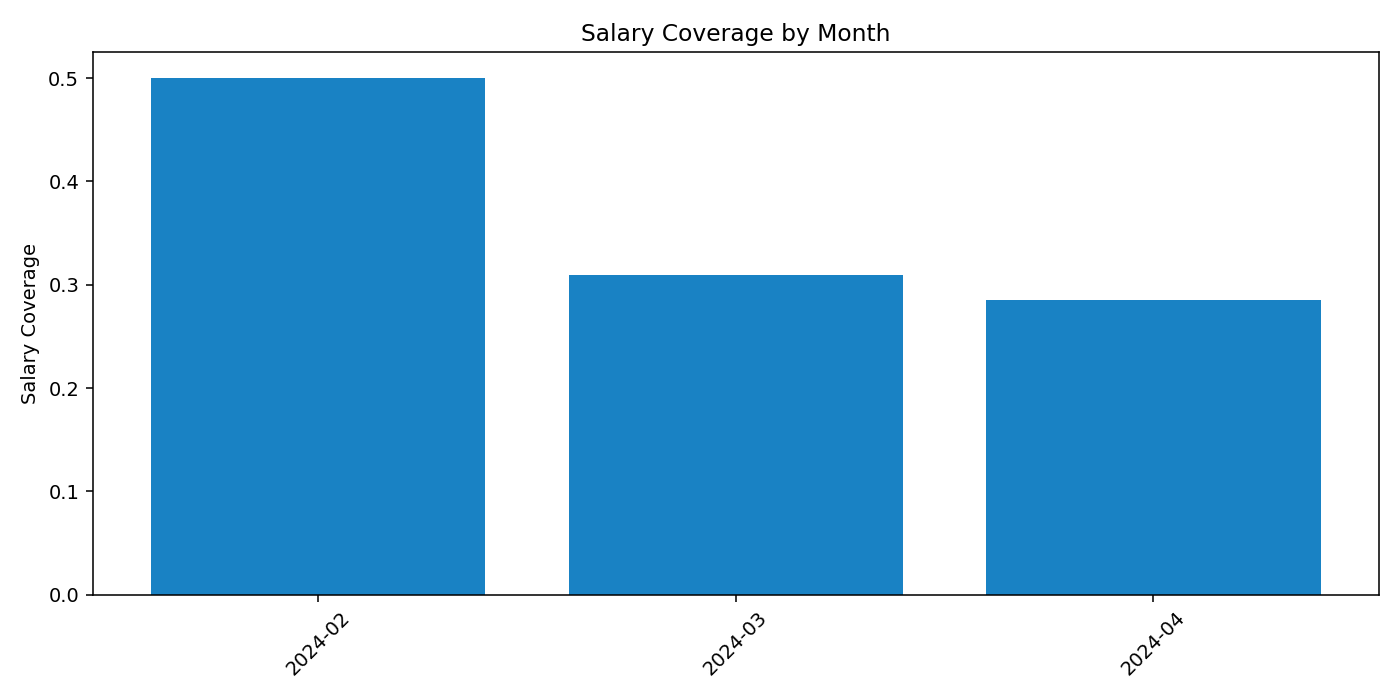
\includegraphics[width=\linewidth]{salary_coverage_by_month.png}\\
      \footnotesize Cobertura de salario por día (solo $\sim$29\% de las filas).
    \end{column}
    \begin{column}{0.5\textwidth}
      \centering
      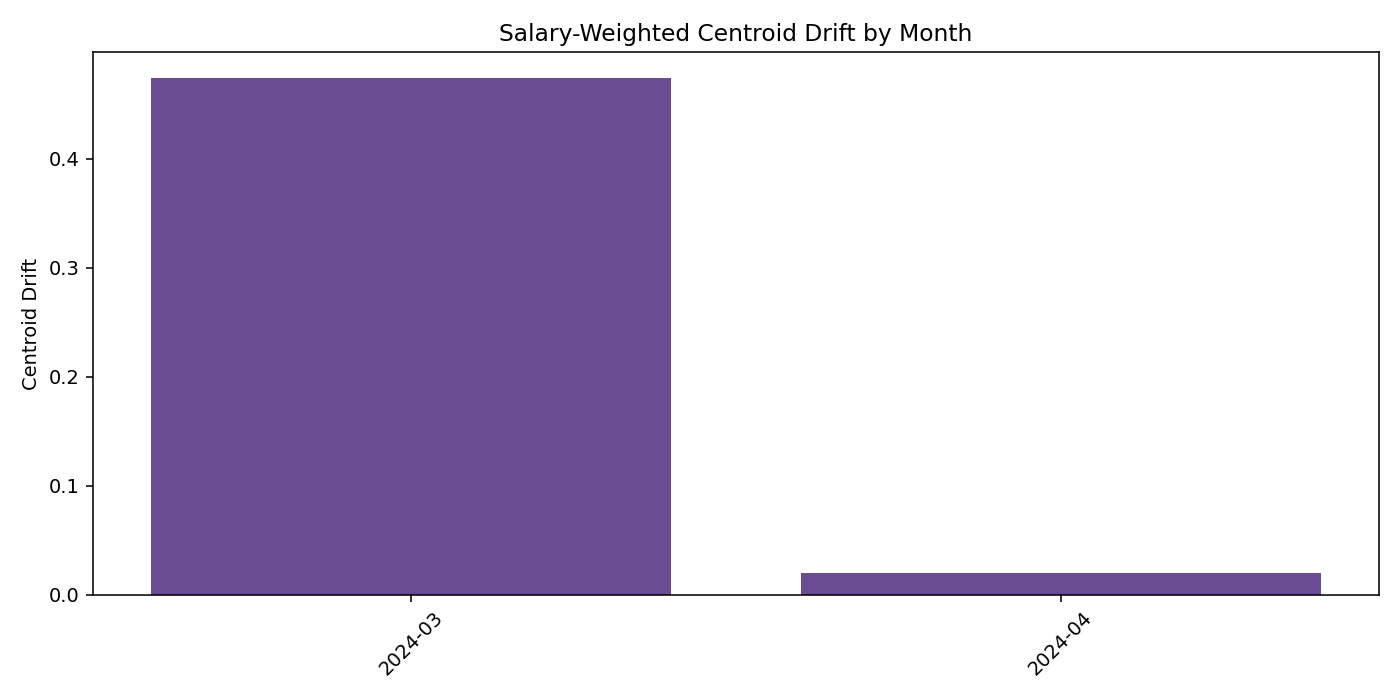
\includegraphics[width=\linewidth]{centroid_drift_salary_weighted_by_month.png}\\
      \footnotesize Deriva de centroides ponderada por salario (subset USD).
    \end{column}
  \end{columns}
\end{frame}

% ------------------------------------------------------------------ %
\section{Hacia mejores modelos}

\begin{frame}{Uso de mejores modelos}
  \centering
  \small
  \begin{tabular}{llll}
    \toprule
    Nivel & Modelo & Representación & Hardware \\
    \midrule
    M0--M1 & TF-IDF / SVD & disperso (30--60k vocab) & CPU 6\,GB \\
    M2 & Qwen3-Embedding-0.6B & denso 1536-dim & GPU T4 \\
    M3 (roadmap) & Qwen3-8B / vLLM & extracción de skills & GPU \\
    M4 (roadmap) & --- & métricas de evaluación & --- \\
    \bottomrule
  \end{tabular}
  \vfill
  \begin{columns}[T]
    \begin{column}{0.5\textwidth}
      \textbf{Por qué mejores modelos}
      \begin{itemize}
        \item TF-IDF no capta sinónimos ni contexto.
        \item Embeddings densos mejoran similitud semántica y clustering.
      \end{itemize}
    \end{column}
    \begin{column}{0.5\textwidth}
      \textbf{Trade-off}
      \begin{itemize}
        \item Más calidad $\Rightarrow$ más cómputo (GPU) y almacenamiento.
        \item Esto motiva el frente de costos.
      \end{itemize}
    \end{column}
  \end{columns}
\end{frame}

\begin{frame}{Evolución de skills por dominio}
  \begin{columns}[T]
    \begin{column}{0.5\textwidth}
      \centering
      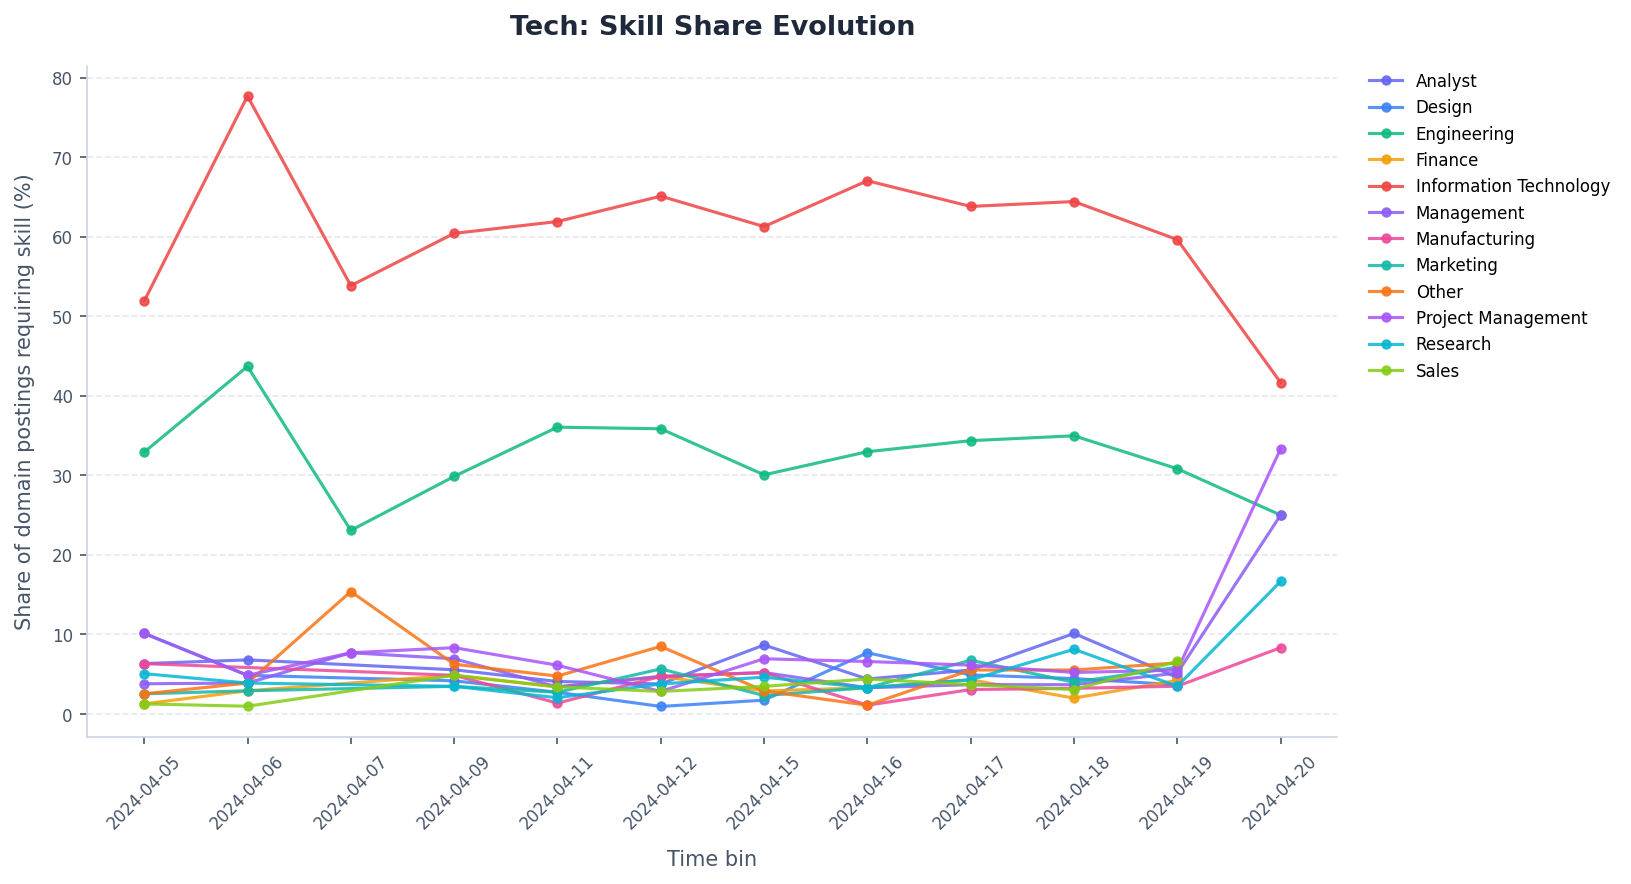
\includegraphics[width=\linewidth]{skill_evolution_tech.png}\\
      \footnotesize Tech
    \end{column}
    \begin{column}{0.5\textwidth}
      \centering
      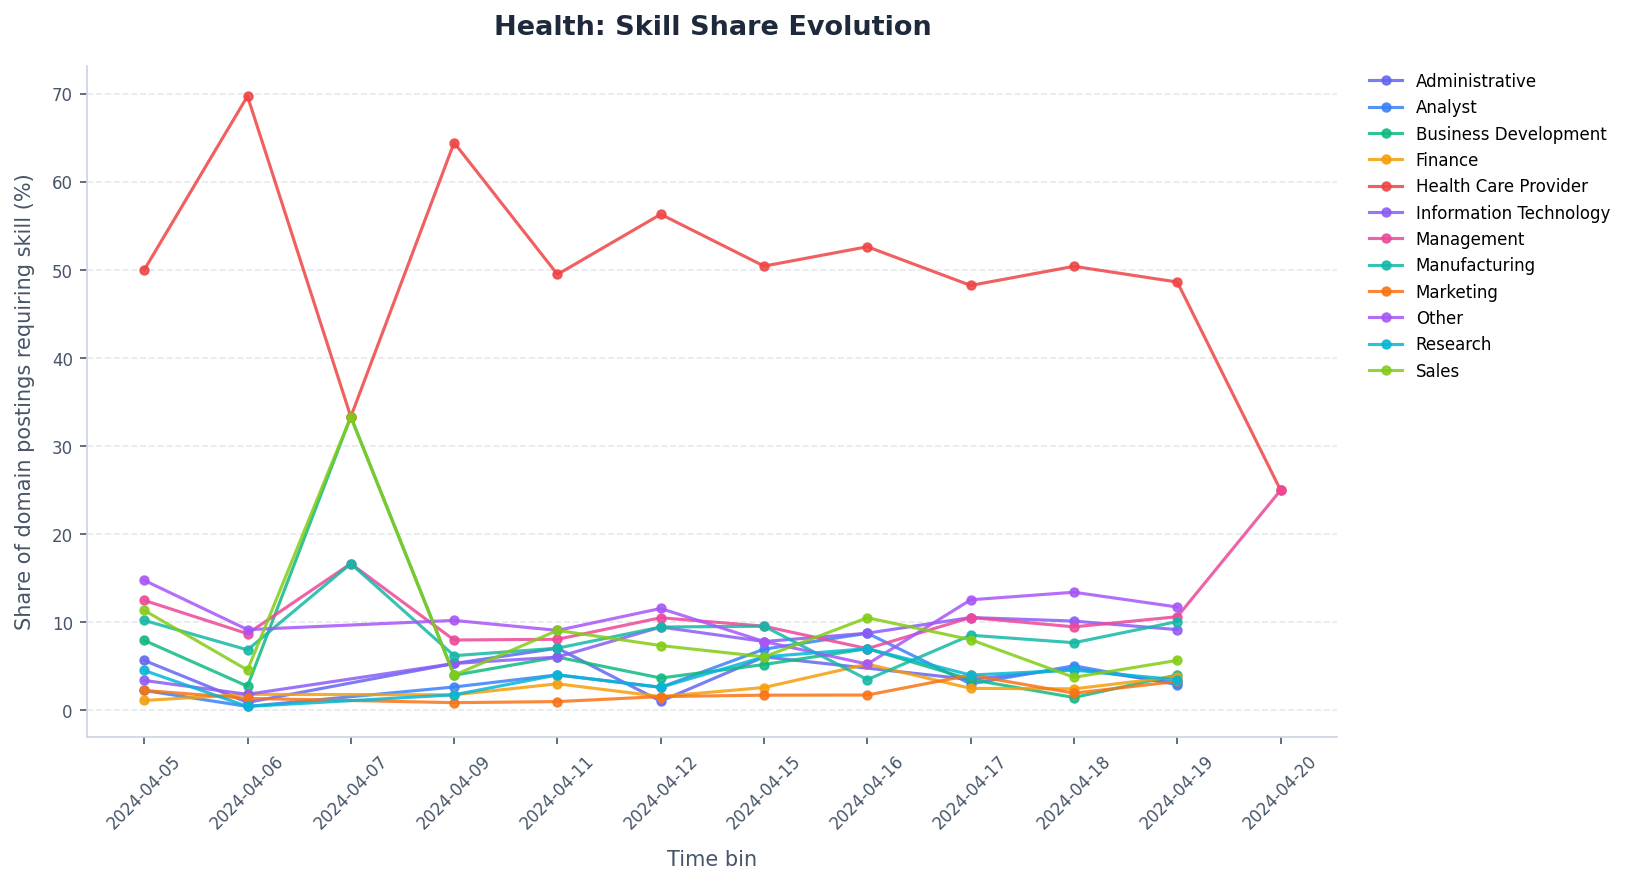
\includegraphics[width=\linewidth]{skill_evolution_health.png}\\
      \footnotesize Salud
    \end{column}
  \end{columns}
\end{frame}

% ------------------------------------------------------------------ %
\section{Frente nuevo: almacenamiento y costos AWS}

\begin{frame}{Motivación: ¿cuántos TB y a qué costo?}
  \begin{itemize}
    \item Más datos + mejores modelos $\Rightarrow$ más almacenamiento y más
          cómputo.
    \item Objetivo: \textbf{estimar TB necesarios} según el crecimiento del
          proyecto y \textbf{proyectar el costo AWS}.
    \item Modelo parametrizado (\texttt{scripts/aws\_cost\_projection.py}):
      \begin{itemize}
        \item $\sim$12\,KB/job (raw 4.3 + embedding 6 + overhead 2).
        \item Base: 123.849 jobs/mes; escenarios 0\% / 5\% / 12\% MoM.
      \end{itemize}
  \end{itemize}
\end{frame}

\begin{frame}{Crecimiento de almacenamiento (TB)}
  \centering
  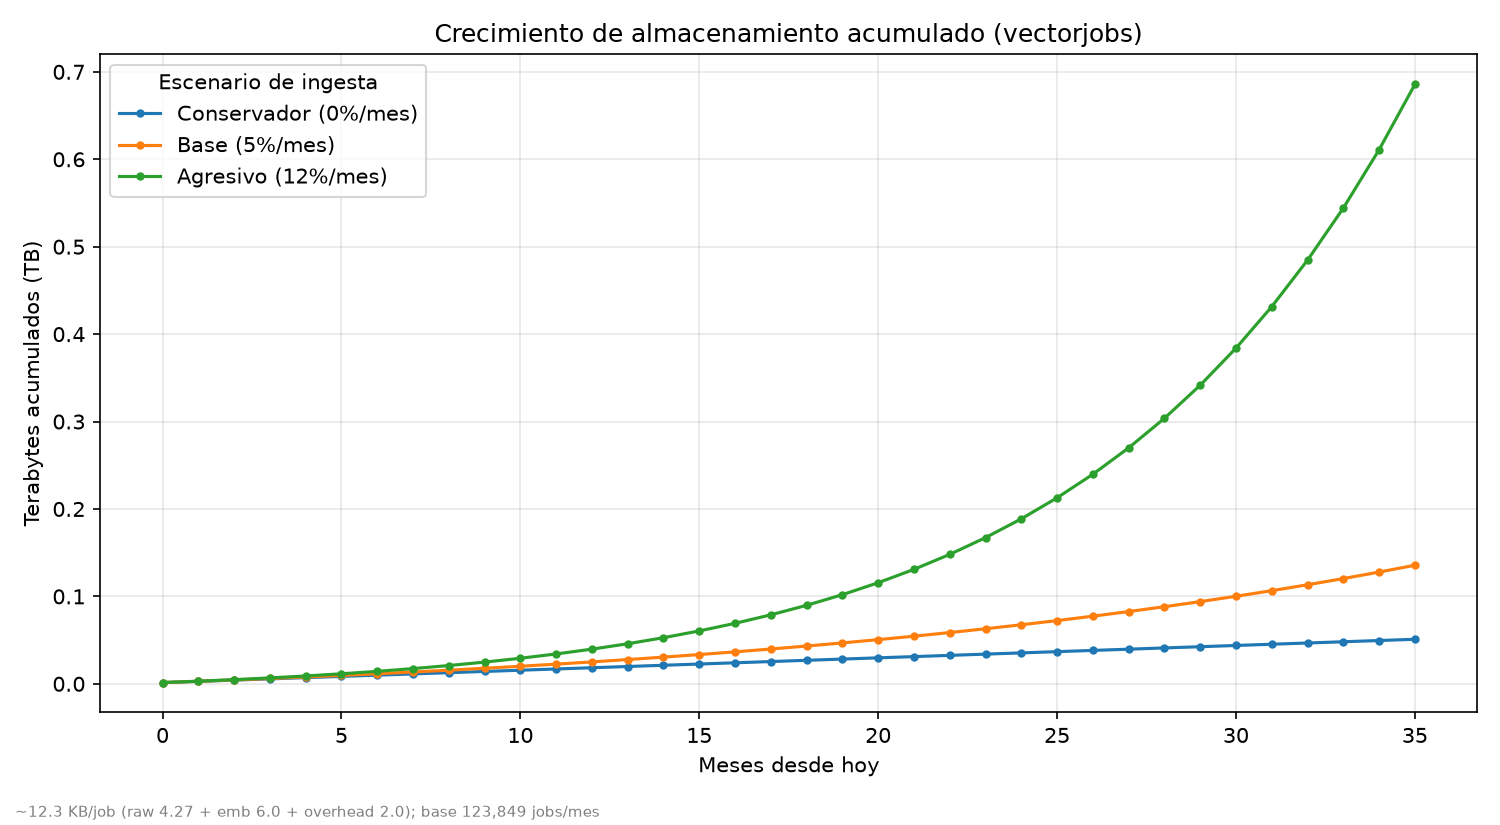
\includegraphics[width=0.82\linewidth]{storage_growth_tb.png}\\
  \footnotesize TB acumulados a 36 meses según el ritmo de ingesta. El factor
  por job y la tasa de crecimiento son parámetros editables.
\end{frame}

\begin{frame}{Precios AWS reales y cambios mensuales}
  \begin{columns}[T]
    \begin{column}{0.5\textwidth}
      \textbf{Almacenamiento --- S3 Standard (us-east-1)}
      \begin{itemize}
        \item \$0.023/GB-mes (primeros 50 TB)
        \item \$0.022 (siguientes 450 TB)
        \item \$0.021 (>500 TB)
      \end{itemize}
      \vspace{0.5em}
      \textbf{Cómputo --- GPU EC2}
      \begin{itemize}
        \item $-45\%$ jun-2025 (p5.48xlarge \$3.86$\rightarrow$\$2.16/h)
        \item $+15\%$ ene-2026 (H200 capacity blocks)
      \end{itemize}
    \end{column}
    \begin{column}{0.5\textwidth}
      \begin{itemize}
        \item El precio del cómputo \textbf{no} baja de forma monótona: cambia
              mes a mes según oferta/demanda de GPUs.
        \item Conviene seguir el precio mensual y comparar antes de
              re-embeddear todo el corpus.
      \end{itemize}
      \vspace{0.3em}
      \footnotesize Fuentes: nops.io / cloudzero (S3 2026); cloudoptimo
      (recorte jun-2025); theregister / itpro (alza ene-2026).
    \end{column}
  \end{columns}
\end{frame}

\begin{frame}{Proyección de costo mensual (S3 + cómputo)}
  \centering
  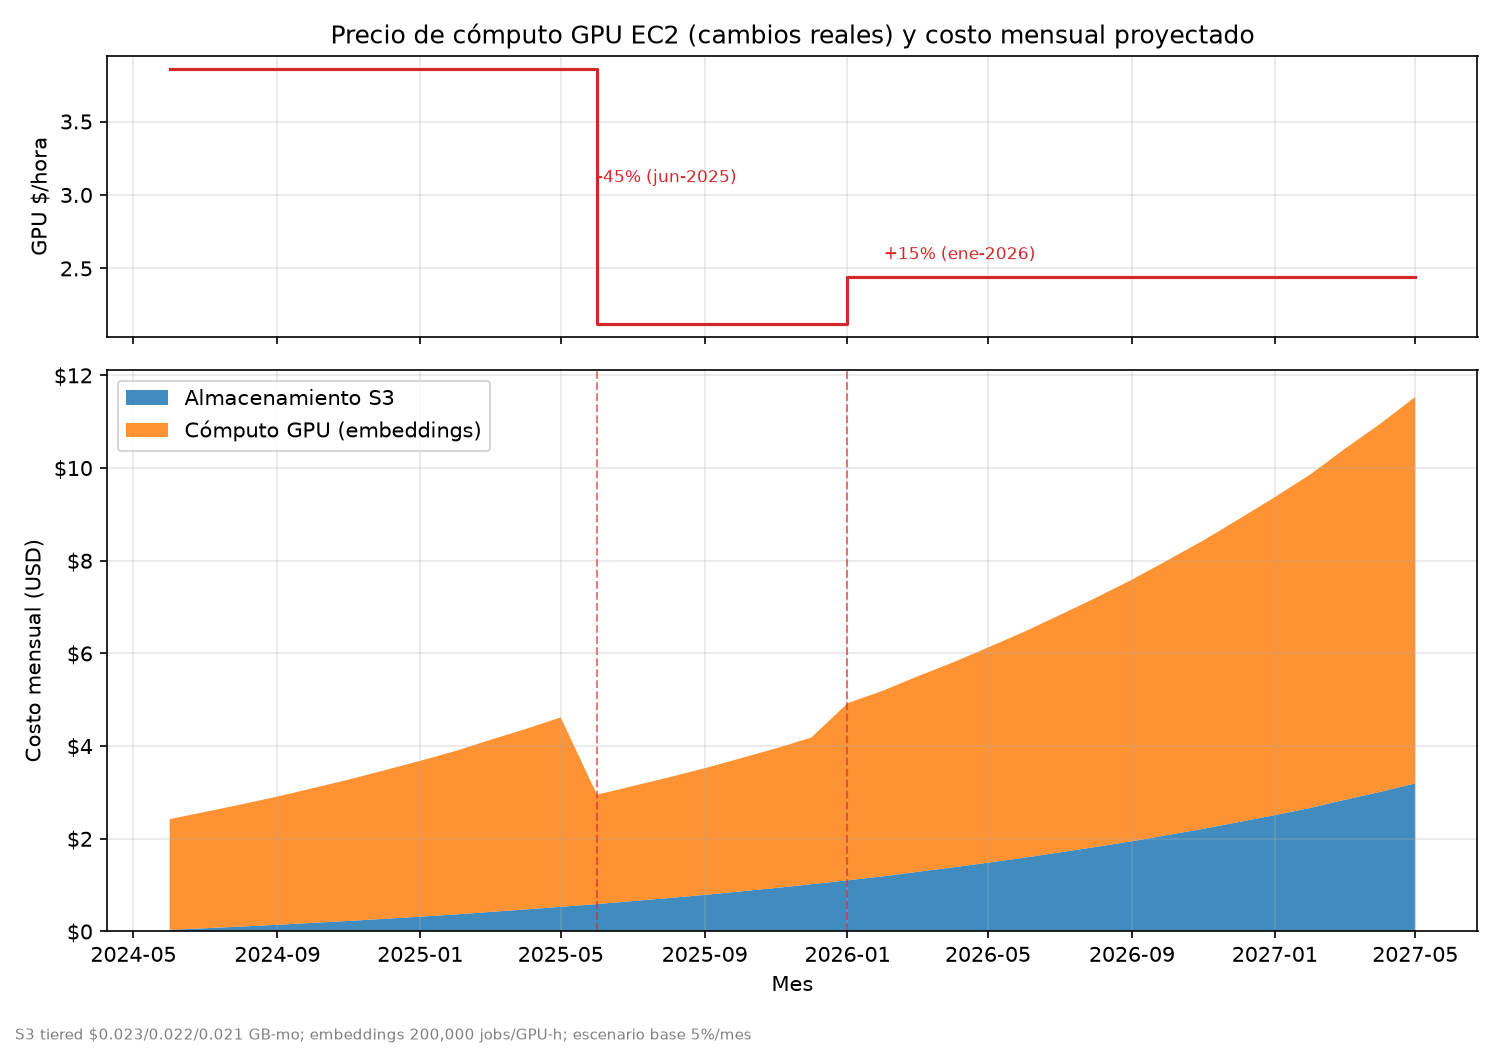
\includegraphics[width=0.86\linewidth]{aws_cost_projection.png}\\
  \footnotesize Costo mensual proyectado (escenario base). Las líneas rojas
  marcan los cambios reales de precio de GPU.
\end{frame}

% ------------------------------------------------------------------ %
\section{Cierre}

\begin{frame}{Conclusiones y próximos pasos}
  \begin{itemize}
    \item \textbf{Centroides}: capturan y siguen la deriva de cada sector en el
          tiempo; base de toda la analítica temporal.
    \item \textbf{Valor de mercado}: volumen $\times$ salario da un proxy de
          "market cap" por sector --- pendiente recalcular con datos completos.
    \item \textbf{Mejores modelos}: TF-IDF $\rightarrow$ Qwen3 $\rightarrow$
          M3/M4; mejoran calidad a costa de cómputo.
    \item \textbf{Costos AWS}: modelo parametrizado de TB y costo con precios
          reales; el cómputo GPU es volátil mes a mes.
  \end{itemize}
  \vfill
  \footnotesize PoC de datos en la nube: \texttt{scripts/download\_dataset.py}
  descarga el dataset de Kaggle y genera un sample pequeño reproducible.
\end{frame}

\end{document}
